% Provenance (never printed): cycle 4 SVT, "La planete Terre": the dynamics of
% the Earth's outer shell, plates and their boundaries, continental drift as a
% history of ideas; see sources/outline_sources.md. Pilot chapter, 2026-10-22.
\chapter{Tektonika Lempeng: Teka-teki yang Bergerak}\label{ch:g7:plate-tectonics}

Bentangkan \omterm{def:g3:continents-and-oceans:world-map}{peta dunia} di atas meja dan perhatikan kedua pantai \omterm{def:g2:water-on-earth:ocean}{Samudra}
Atlantik. Tonjolan besar Brasil seolah-olah dibuat untuk masuk ke lekukan
pantai barat Afrika, seakan-akan seseorang telah memotong sebongkah daratan
menjadi dua lalu mendorong kedua belahannya saling menjauh. Orang-orang
pertama yang mencetak \omterm{def:g2:drawing-to-map:map}{peta} yang baik dari kedua pantai itu langsung
menyadarinya. Selama tiga abad hal itu tetap menjadi keanehan saja. Pada
abad kedua puluh, keanehan itu menjadi titik awal teori yang kini
menjelaskan mengapa tanah berguncang di Jepang, mengapa \omterm{def:g4:world-physical-map:range}{Pegunungan} Andes
begitu tinggi, mengapa Islandia perlahan-lahan makin lebar --- dan mengapa
\omterm{def:g2:drawing-to-map:map}{peta} di atas meja hanyalah potret sesaat dari dunia yang sedang bergerak.

\begin{omfigure}
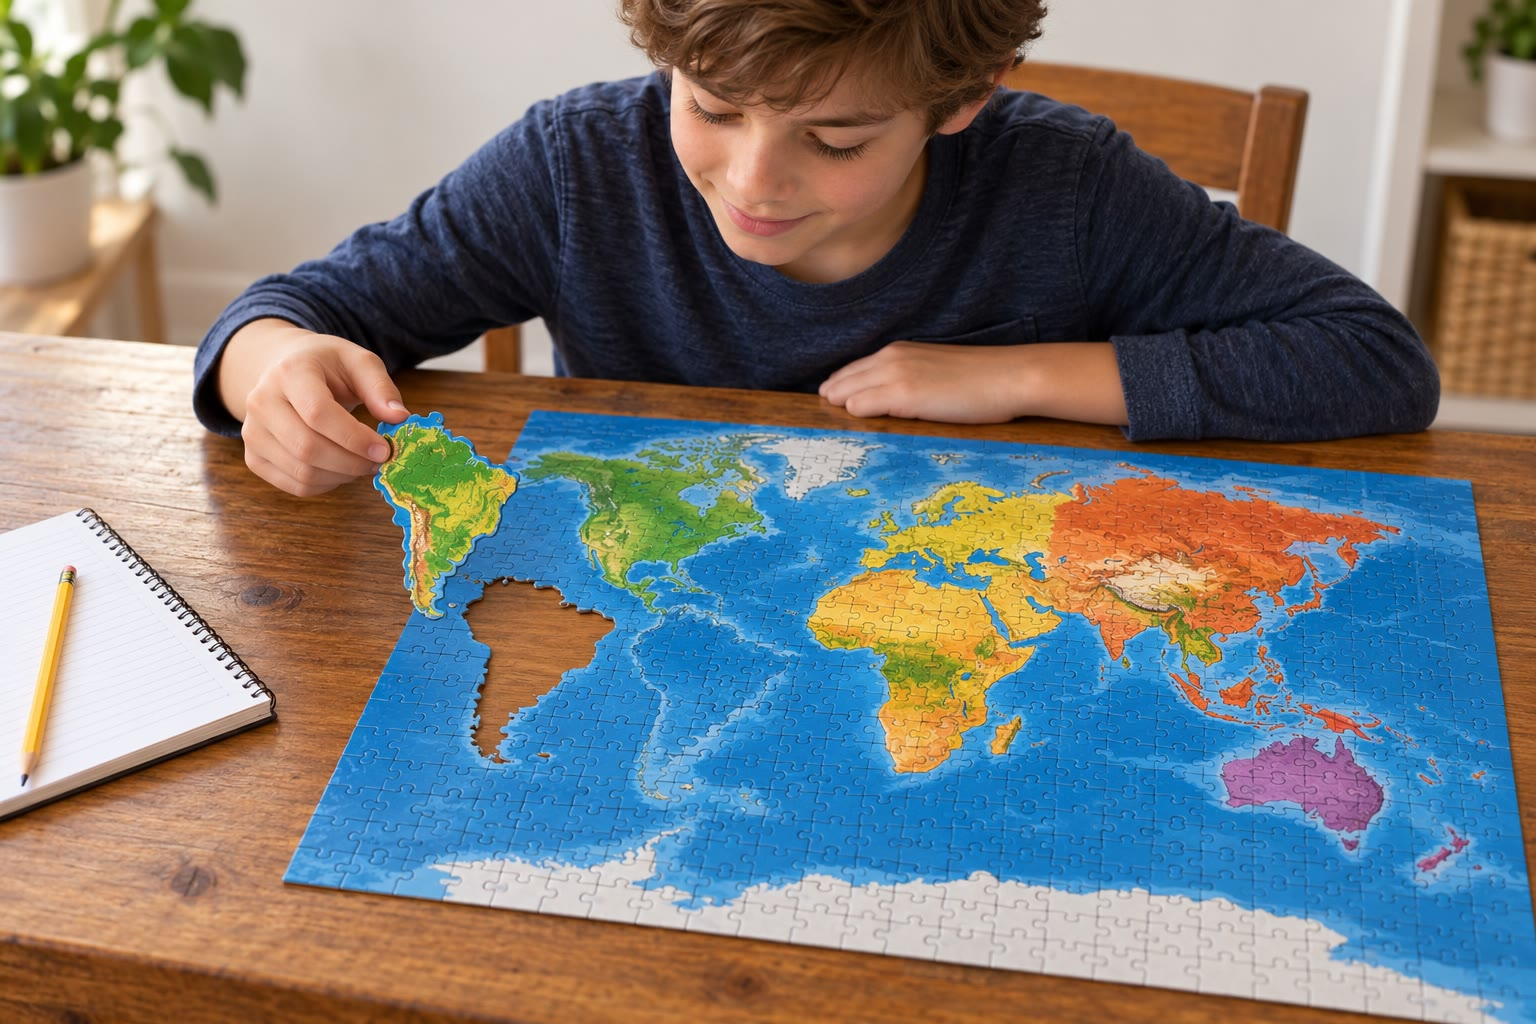
\includegraphics[width=0.62\linewidth]{images/book1/ai/g7-puzzle-map.jpg}

{\small Amerika Selatan di samping Afrika: pada sebuah puzzle, kecocokannya
hanyalah permainan; pada Bumi yang sesungguhnya, kecocokan itu adalah petunjuk.}
\end{omfigure}

\begin{recall}
Bumi mempunyai tiga lapisan utama: \emph{\omterm{def:g6:inside-the-earth:layers}{kerak}} \omterm{def:g3:stones-pebbles-sand:rock}{batuan} yang tipis,
\emph{\omterm{def:g6:inside-the-earth:layers}{mantel}} \omterm{def:g3:stones-pebbles-sand:rock}{batuan} panas yang tebal, dan \emph{\omterm{def:g6:inside-the-earth:layers}{inti}} dari logam; suhu
naik seiring kedalaman (\cref{ch:g6:inside-the-earth}). Sebuah tempat di
\omterm{def:g3:continents-and-oceans:globe}{bola dunia} ditentukan oleh \omterm{def:g6:latitude-longitude:latitude}{lintang} dan \omterm{def:g6:latitude-longitude:longitude}{bujurnya} (\cref{ch:g6:latitude-longitude}).
\end{recall}

\section{Benua-benua yang dulu saling cocok}

\begin{definition}[Pergeseran benua]\label{def:g7:plate-tectonics:continental-drift}
Yang disebut \emph{pergeseran benua}\index{pergeseran benua} adalah gagasan
bahwa \omterm{def:g3:continents-and-oceans:continent}{benua-benua} bergerak perlahan di permukaan Bumi, sehingga letaknya,
dan bentuk \omterm{def:g2:water-on-earth:ocean}{samudra} di antaranya, telah berubah dari zaman ke zaman.
\end{definition}

\begin{definition}[Superbenua]\label{def:g7:plate-tectonics:supercontinent}
Yang disebut \emph{superbenua}\index{superbenua} adalah satu daratan tunggal
yang terdiri atas semua, atau hampir semua, \omterm{def:g3:continents-and-oceans:continent}{benua} yang menyatu. Superbenua
yang terakhir, \emph{Pangea}\index{Pangea} (``semua daratan'' dalam bahasa
Yunani), mulai terpecah antara kira-kira 225 dan 200 juta tahun yang lalu.
% ledger: usgs:pangaea-breakup
\end{definition}

Ilmuwan yang membela \omterm{def:g7:plate-tectonics:continental-drift}{pergeseran benua} sebagai teori yang sungguh-sungguh,
dengan bukti, adalah Alfred Wegener. Ia mengumpulkan empat jenis petunjuk.

\begin{enumerate}
  \item \textbf{Bentuk pantai.} Amerika Selatan dan Afrika saling cocok
        seperti dua keping puzzle, demikian pula beberapa garis pantai
        lainnya.
  \item \textbf{Fosil.} Fosil hewan dan tumbuhan yang sama ditemukan di
        \omterm{def:g3:continents-and-oceans:continent}{benua-benua} yang kini dipisahkan oleh \omterm{def:g2:water-on-earth:ocean}{samudra} selebar ribuan
        kilometer. \emph{Mesosaurus} adalah reptil kecil yang hidup di \omterm{def:g2:water-on-earth:salt-fresh}{air
        tawar}: hewan itu tidak mungkin berenang menyeberangi \omterm{def:g2:water-on-earth:ocean}{samudra}, tetapi
        fosilnya terdapat di Brasil dan juga di Afrika bagian selatan.
  \item \textbf{\omterm{def:g3:stones-pebbles-sand:rock}{Batuan}.} \omterm{def:g3:stones-pebbles-sand:rock}{Batuan} yang jenis dan umurnya sama, serta
        \omterm{def:g4:world-physical-map:range}{pegunungan} tua yang bentuknya sama, berhenti di satu pantai lalu
        berlanjut lagi di pantai seberangnya, seperti baris-baris tulisan
        pada koran yang robek.
  \item \textbf{\omterm{def:g5:weather-and-climate:climate}{Iklim} purba.} Batu bara, yang terbentuk dari tumbuhan hutan
        rawa yang hangat, ditemukan di Antarktika; jejak yang ditinggalkan
        gletser purba ditemukan di bagian Afrika yang kini panas dan kering.
        Daratan ini pasti dulu berada di \omterm{def:g5:weather-and-climate:climate}{iklim} lain, pada \omterm{def:g6:latitude-longitude:latitude}{lintang} yang lain.
\end{enumerate}
% ledger: usgs:coal-antarctica, usgs:fossil-map

\begin{omfigure}
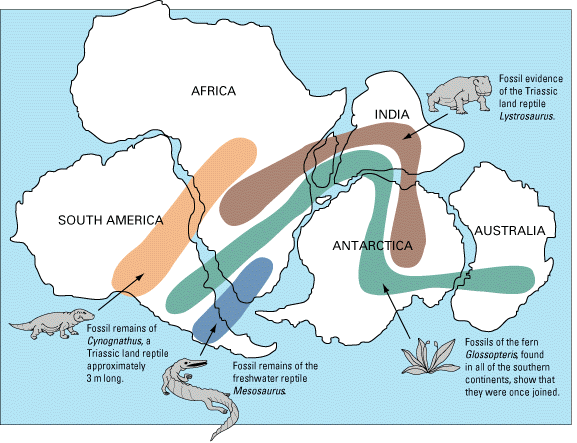
\includegraphics[width=0.86\linewidth]{images/book1/g7-usgs-fossil-map.png}

{\small \omterm{def:g3:continents-and-oceans:continent}{Benua-benua} selatan disatukan kembali. Setiap pita berwarna
menghubungkan tempat-tempat ditemukannya satu spesies fosil pada masa kini:
reptil darat \emph{Cynognathus} dan \emph{Lystrosaurus}, reptil \omterm{def:g2:water-on-earth:salt-fresh}{air tawar}
\emph{Mesosaurus}, dan tumbuhan paku \emph{Glossopteris}. Jika \omterm{def:g3:continents-and-oceans:continent}{benua-benua}
itu terpisah, pita-pitanya tercerai-berai; jika disatukan, pita-pita itu
bersambung tanpa terputus. \omterm{def:g2:drawing-to-map:map}{Peta}: U.S. Geological Survey, \emph{This Dynamic
Earth} (domain publik).}
\end{omfigure}

\begin{history}[Gagasan Wegener, 1912--1930]
% ledger: usgs:wegener-1912, usgs:wegener-death, usgs:jeffreys
Alfred Wegener, seorang ahli meteorologi Jerman berusia 32 tahun,
memaparkan teori \omterm{def:g7:plate-tectonics:continental-drift}{pergeseran benua} dalam dua artikel pada tahun 1912.
Sebagian besar ahli geologi menolaknya. Keberatan yang paling kuat adalah
bahwa Wegener tidak dapat mengatakan \emph{apa} yang menggerakkan \omterm{def:g3:continents-and-oceans:continent}{benua}:
ia mengira \omterm{def:g3:continents-and-oceans:continent}{benua-benua} itu membajak \omterm{def:g3:stones-pebbles-sand:rock}{batuan dasar} \omterm{def:g2:water-on-earth:ocean}{samudra}, dan ahli fisika
Harold Jeffreys menunjukkan bahwa \omterm{def:g3:continents-and-oceans:continent}{benua} yang padat tidak mungkin melakukan
hal itu tanpa hancur. Wegener terus mengumpulkan bukti sampai ia meninggal
di lapisan es Greenland pada tahun 1930, dalam sebuah ekspedisi. Jawaban
yang tidak dimilikinya datang dari dasar \omterm{def:g2:water-on-earth:ocean}{samudra}, yang dijelajahi sesudah
tahun 1950-an: kisahnya diceritakan pada tahun ajaran berikutnya.
\end{history}

\section{Lempeng-lempeng}

Petunjuk-petunjuk Wegener benar, tetapi \omterm{def:g3:continents-and-oceans:continent}{benua-benuanya} adalah kepingan yang
salah. Bukan hanya \omterm{def:g3:continents-and-oceans:continent}{benua} yang bergerak: seluruh cangkang luar Bumi, di
bawah \omterm{def:g3:continents-and-oceans:continent}{benua} maupun di bawah \omterm{def:g2:water-on-earth:ocean}{samudra}, terpecah menjadi kepingan-kepingan.

\begin{definition}[Lempeng tektonik]\label{def:g7:plate-tectonics:plate}
Yang disebut \emph{lempeng tektonik}\index{lempeng tektonik} (atau singkatnya
lempeng) adalah bongkah \omterm{def:g3:stones-pebbles-sand:rock}{batuan} yang besar dan kaku, yang menjadi bagian
dari cangkang luar Bumi. Lempeng terdiri atas \omterm{def:g6:inside-the-earth:layers}{kerak} dan bagian teratas
\omterm{def:g6:inside-the-earth:layers}{mantel} yang dingin dan kaku, yang bersama-sama tebalnya rata-rata paling
sedikit 80 kilometer; lempeng itu bergerak perlahan di atas \omterm{def:g6:inside-the-earth:layers}{mantel} di
bawahnya yang lebih panas dan lebih lunak.
% ledger: usgs:lithosphere-80km
\end{definition}

\begin{definition}[Tektonika lempeng]\label{def:g7:plate-tectonics:plate-tectonics}
Yang disebut \emph{tektonika lempeng}\index{tektonika lempeng} adalah teori
bahwa cangkang luar Bumi terbagi menjadi \omterm{def:g7:plate-tectonics:plate}{lempeng-lempeng} yang bergerak
relatif satu terhadap yang lain, dan bahwa sebagian besar \omterm{def:g4:volcanoes-earthquakes-first-look:earthquake}{gempa bumi}, \omterm{def:g4:volcanoes-earthquakes-first-look:volcano}{gunung
api}, dan \omterm{def:g4:world-physical-map:range}{pegunungan} terbentuk di tempat \omterm{def:g7:plate-tectonics:plate}{lempeng-lempeng} itu bertemu.
\end{definition}

\begin{remark}[Berapa banyak lempeng?]\label{rem:g7:plate-tectonics:how-many}
% ledger: usgs:plates-dozen, pb2002:count
Kira-kira selusin \omterm{def:g7:plate-tectonics:plate}{lempeng} berukuran besar; jauh lebih banyak lagi yang
kecil. Sebuah \omterm{def:g2:drawing-to-map:map}{peta} terperinci yang dipakai para ahli geologi menghitung 52
\omterm{def:g7:plate-tectonics:plate}{lempeng}. Sebuah \omterm{def:g7:plate-tectonics:plate}{lempeng} dapat membawa \omterm{def:g3:continents-and-oceans:continent}{benua}, \omterm{def:g2:water-on-earth:ocean}{samudra}, atau keduanya:
\omterm{def:g7:plate-tectonics:plate}{lempeng} Amerika Selatan membawa seluruh Amerika Selatan dan separuh barat
\omterm{def:g2:water-on-earth:ocean}{Samudra} Atlantik Selatan. \omterm{def:g7:plate-tectonics:plate}{Lempeng} Pasifik, yang terbesar, hampir tidak
membawa daratan sama sekali.
\end{remark}

\begin{omfigure}
\begin{tikzpicture}
\begin{axis}[ommap, width=\linewidth, xtick={-180,-90,...,180}, ytick={-60,0,60}]
\addplot[fill=omLithAlluv, draw=black!45, line width=0.2pt] table {figdata/out/shared-geo-land.dat};
\addplot[omRidge, line width=0.8pt] table {figdata/out/shared-geo-school-ridge.dat};
\addplot[omRidge!70!black, line width=0.8pt] table {figdata/out/shared-geo-school-transform.dat};
\addplot[omTrench, line width=0.8pt] table {figdata/out/shared-geo-school-subduction.dat};
\addplot[fill=omTrench, draw=none] table {figdata/out/shared-geo-school-teeth.dat};
\addplot[black!65, line width=0.8pt] table {figdata/out/shared-geo-school-collision.dat};
\begin{scope}[every node/.style={font=\scriptsize\bfseries, text=black!85,
    fill=white, fill opacity=0.75, text opacity=1, inner sep=1pt, align=center}]
  \node at (axis cs:-150,12) {Pasifik};
  \node at (axis cs:-103,52) {Amerika\\Utara};
  \node at (axis cs:-48,-12) {Amerika\\Selatan};
  \node at (axis cs:85,57) {Eurasia};
  \node at (axis cs:18,8) {Afrika};
  \node at (axis cs:10,-75) {Antarktika};
  \node at (axis cs:78,11) {India};
  \node at (axis cs:128,-26) {Australia};
  \node at (axis cs:-95,-22) {Nazca};
  \node at (axis cs:50,20) {Arab};
\end{scope}
\end{axis}
\end{tikzpicture}

{\small \omterm{def:g7:plate-tectonics:plate}{Lempeng-lempeng} tektonik utama. Merah: \omterm{def:g7:plate-tectonics:plate}{lempeng} yang saling menjauh;
biru dengan segitiga: satu \omterm{def:g7:plate-tectonics:plate}{lempeng} menunjam ke bawah \omterm{def:g7:plate-tectonics:plate}{lempeng} yang lain
(segitiganya berada pada \omterm{def:g7:plate-tectonics:plate}{lempeng} yang tetap di atas); abu-abu: \omterm{def:g7:plate-tectonics:plate}{lempeng} yang
saling mendorong pada zona \omterm{def:g4:world-physical-map:range}{pegunungan} yang lebar; merah tua: \omterm{def:g7:plate-tectonics:plate}{lempeng} yang
saling bergeser berpapasan. \omterm{def:g7:plate-tectonics:plate-boundary}{Batas lempeng} menurut P.~Bird (2003); garis
pantai dari Natural Earth.}
\end{omfigure}

Bagaimana kita mengetahui di mana satu \omterm{def:g7:plate-tectonics:plate}{lempeng} berakhir dan \omterm{def:g7:plate-tectonics:plate}{lempeng}
berikutnya dimulai? Lihatlah tempat-tempat yang Buminya gelisah.

\begin{proposition}[Gempa bumi dan gunung api menelusuri batas lempeng]\label{prop:g7:plate-tectonics:restless}
% ledger: data:usgs-comcat, data:pb2002 (share computed in figdata/grade-7/quakes_on_boundaries.py)
\omterm{def:g4:volcanoes-earthquakes-first-look:earthquake}{Gempa bumi} dan \omterm{def:g4:volcanoes-earthquakes-first-look:volcano}{gunung api} tidak tersebar secara acak di Bumi: sebagian
besar terletak di sepanjang sabuk-sabuk yang sempit, dan sabuk-sabuk ini
adalah tepi \omterm{def:g7:plate-tectonics:plate}{lempeng}. Dari 7\,031 \omterm{def:g4:volcanoes-earthquakes-first-look:earthquake}{gempa bumi} bermagnitudo 6 atau lebih yang
tercatat antara tahun 1976 dan 2025, 6\,472 --- yaitu 92\,\% --- terjadi
kurang dari \qty{300}{km} dari sebuah \omterm{def:g7:plate-tectonics:plate-boundary}{batas lempeng}.
\end{proposition}

\begin{omfigure}
\begin{tikzpicture}
\begin{axis}[ommap, width=\linewidth, xtick={-180,-90,...,180}, ytick={-60,0,60},
  legend style={at={(0.02,0.04)}, anchor=south west, font=\scriptsize,
  fill=white, fill opacity=0.85, text opacity=1, draw=black!40}]
\addplot[fill=omLithAlluv, draw=black!45, line width=0.2pt, forget plot] table {figdata/out/shared-geo-land.dat};
\addplot[only marks, mark=*, mark size=0.45pt, omThm!85!black] table[x=lon, y=lat] {figdata/out/grade-7-quakes_on_boundaries-map.dat};
\addlegendentry{gempa bumi, magnitudo 6.5 atau lebih, 1976--2025}
\addplot[only marks, mark=triangle*, mark size=1.1pt, black] table {figdata/out/shared-geo-volcanoes.dat};
\addlegendentry{gunung api yang aktif dalam 12\,000 tahun terakhir}
\end{axis}
\end{tikzpicture}

{\small \omterm{def:g4:volcanoes-earthquakes-first-look:earthquake}{Gempa bumi} besar dan \omterm{def:g4:volcanoes-earthquakes-first-look:volcano}{gunung api} muda. Bandingkan dengan \omterm{def:g2:drawing-to-map:map}{peta}
\omterm{def:g7:plate-tectonics:plate}{lempeng} di atas: titik-titik dan segitiga-segitiga itu menggambar \omterm{def:g7:plate-tectonics:plate-boundary}{batas
lempeng}. Data: katalog \omterm{def:g4:volcanoes-earthquakes-first-look:earthquake}{gempa bumi} U.S. Geological Survey; Smithsonian Global
Volcanism Program.}
\end{omfigure}

\section{Tiga jenis batas lempeng}

\begin{definition}[Batas lempeng]\label{def:g7:plate-tectonics:plate-boundary}
Yang disebut \emph{batas lempeng}\index{batas lempeng} adalah garis, atau
zona sempit, tempat dua \omterm{def:g7:plate-tectonics:plate}{lempeng} bertemu. Menurut cara kedua \omterm{def:g7:plate-tectonics:plate}{lempeng} itu
bergerak terhadap satu sama lain, sebuah batas termasuk salah satu dari
tiga jenis:
\begin{itemize}
  \item pada \emph{batas divergen}\index{batas divergen} kedua \omterm{def:g7:plate-tectonics:plate}{lempeng}
        saling menjauh;
  \item pada \emph{batas konvergen}\index{batas konvergen} kedua \omterm{def:g7:plate-tectonics:plate}{lempeng}
        saling mendekat;
  \item pada \emph{batas transform}\index{batas transform} kedua \omterm{def:g7:plate-tectonics:plate}{lempeng}
        saling bergeser berpapasan, berdampingan.
\end{itemize}
\end{definition}

\begin{example}[Batas divergen: Islandia dan Afrika Timur]\label{ex:g7:plate-tectonics:divergent}
% ledger: usgs:iceland, usgs:east-africa
Di tengah-tengah \omterm{def:g2:water-on-earth:ocean}{Samudra} Atlantik membentang rangkaian \omterm{def:g4:world-physical-map:range}{pegunungan} bawah
\omterm{def:g2:water-on-earth:ocean}{laut}, Punggung Tengah Atlantik, tempat \omterm{def:g7:plate-tectonics:plate}{lempeng-lempeng} di kedua sisinya
saling menjauh. \omterm{def:g3:stones-pebbles-sand:rock}{Batuan} panas dari \omterm{def:g6:inside-the-earth:layers}{mantel} naik ke celah itu, sebagian
meleleh, dan menjadi dasar \omterm{def:g2:water-on-earth:ocean}{laut} yang baru: \omterm{def:g7:plate-tectonics:plate-boundary}{batas divergen} membangun \omterm{def:g7:plate-tectonics:plate}{lempeng}
baru. Islandia adalah bagian punggung ini yang muncul di atas \omterm{def:g2:water-on-earth:ocean}{laut}: di
sana, Amerika Utara bergerak ke barat dan Eurasia ke timur, dan pulau itu
perlahan-lahan terbelah. Antara tahun 1975 dan 1984, retakan-retakan di
dekat \omterm{def:g4:volcanoes-earthquakes-first-look:volcano}{gunung api} Krafla, di utara pulau itu, melebar kira-kira 7 meter
seluruhnya. \omterm{def:g7:plate-tectonics:plate-boundary}{Batas divergen} dapat juga membelah sebuah \omterm{def:g3:continents-and-oceans:continent}{benua}: di sepanjang
Rekahan Afrika Timur, Afrika mulai terbelah, dan \omterm{def:g2:water-on-earth:ocean}{Laut} Merah adalah \omterm{def:g2:water-on-earth:ocean}{samudra}
muda yang sudah memisahkan Arab dari Afrika.
\end{example}

\begin{example}[Batas konvergen: Andes dan Himalaya]\label{ex:g7:plate-tectonics:convergent}
% ledger: usgs:trench-depth, usgs:himalaya
Di lepas pantai barat Amerika Selatan, \omterm{def:g7:plate-tectonics:plate}{lempeng} Nazca, yang membawa
\omterm{def:g2:water-on-earth:ocean}{samudra}, bergerak mendekati \omterm{def:g7:plate-tectonics:plate}{lempeng} Amerika Selatan, yang membawa \omterm{def:g3:continents-and-oceans:continent}{benua}.
\omterm{def:g7:plate-tectonics:plate}{Lempeng} \omterm{def:g2:water-on-earth:ocean}{samudra} itu, yang lebih berat, melengkung dan menunjam ke bawah
\omterm{def:g3:continents-and-oceans:continent}{benua}, jauh ke dalam \omterm{def:g6:inside-the-earth:layers}{mantel}. Di sepanjang garis tempat \omterm{def:g7:plate-tectonics:plate}{lempeng} itu turun,
dasar \omterm{def:g2:water-on-earth:ocean}{laut} menukik ke dalam palung yang dalam; di atas \omterm{def:g7:plate-tectonics:plate}{lempeng} yang
menunjam, daratan diguncang \omterm{def:g4:volcanoes-earthquakes-first-look:earthquake}{gempa bumi} dan dijajari \omterm{def:g4:volcanoes-earthquakes-first-look:volcano}{gunung api}: itulah
\omterm{def:g4:world-physical-map:range}{Pegunungan} Andes. Di Pasifik bagian barat, tempat satu \omterm{def:g7:plate-tectonics:plate}{lempeng} \omterm{def:g2:water-on-earth:ocean}{samudra}
menunjam ke bawah \omterm{def:g7:plate-tectonics:plate}{lempeng} \omterm{def:g2:water-on-earth:ocean}{samudra} lain, palung-palungnya adalah tempat
terdalam di Bumi: Palung Mariana dalamnya hampir \qty{11000}{m}. Ketika
dua \omterm{def:g3:continents-and-oceans:continent}{benua} bertemu, tidak ada yang menunjam: \omterm{def:g6:inside-the-earth:layers}{keraknya} berkerut dan menebal.
India bertabrakan dengan Asia kira-kira 50 juta tahun yang lalu, dan kedua
\omterm{def:g7:plate-tectonics:plate}{lempeng} itu masih saling mendorong; dengan cara itulah Himalaya dan \omterm{def:g1:landscapes-around-us:landform}{Dataran}
Tinggi Tibet terangkat.
\end{example}

\begin{example}[Batas transform: Sesar San Andreas]\label{ex:g7:plate-tectonics:transform}
% ledger: usgs:san-andreas, usgs:san-andreas-photo
Di California, \omterm{def:g7:plate-tectonics:plate}{lempeng} Pasifik bergeser ke arah barat laut melewati \omterm{def:g7:plate-tectonics:plate}{lempeng}
Amerika Utara di sepanjang Sesar San Andreas, yang panjangnya kira-kira
\qty{1300}{km}. Di sana tidak ada \omterm{def:g7:plate-tectonics:plate}{lempeng} yang dibuat atau dihancurkan;
kedua \omterm{def:g7:plate-tectonics:plate}{lempeng} saling bergesekan, dan sentakan-sentakan gesekan itu adalah
\omterm{def:g4:volcanoes-earthquakes-first-look:earthquake}{gempa bumi}.
\end{example}

\begin{omfigure}
\begin{tikzpicture}[x=1cm, y=1cm, font=\small]
  % mantle
  \fill[omLithGranite!45] (0,-3.3) rectangle (12.4,-0.85);
  \node[font=\footnotesize, text=black!75] at (2.6,-2.6) {mantel: panas dan lunak};
  % sea water
  \fill[omSea] (0,0) -- (0,-0.75) -- (1.5,-0.6) -- (3,-0.25) -- (4.5,-0.6)
    -- (7.4,-0.8) -- (8.0,-1.2) -- (8.6,-0.6) -- (8.9,0) -- cycle;
  % oceanic plates (the ridge at x = 3, the trench at x = 8)
  \fill[omLithBasalt!70] (0,-0.75) -- (1.5,-0.6) -- (3,-0.25) -- (4.5,-0.6)
    -- (7.4,-0.8) -- (8.0,-1.2) -- (9.6,-2.3) -- (10.2,-3.3) -- (9.5,-3.3)
    -- (8.6,-2.2) -- (7.5,-1.55) -- (4.5,-1.35) -- (3.2,-0.95) -- (2.8,-0.95)
    -- (1.5,-1.35) -- (0,-1.45) -- cycle;
  % continental plate
  \fill[omLithSand!80] (8.6,-0.6) -- (8.9,0) -- (9.4,0.35) -- (9.8,0.9)
    -- (10.2,0.35) -- (12.4,0.2) -- (12.4,-1.9) -- (10.6,-1.9) -- (9.6,-2.3)
    -- (8.0,-1.2) -- cycle;
  \draw[black!70, line width=0.5pt] (0,-0.75) -- (1.5,-0.6) -- (3,-0.25)
    -- (4.5,-0.6) -- (7.4,-0.8) -- (8.0,-1.2) -- (8.6,-0.6) -- (8.9,0)
    -- (9.4,0.35) -- (9.8,0.9) -- (10.2,0.35) -- (12.4,0.2);
  \draw[black!45, densely dashed] (0,0) -- (8.9,0);
  % magma: under the ridge and under the volcano
  \fill[omThm!80] (2.85,-0.95) -- (3,-0.3) -- (3.15,-0.95) -- cycle;
  \draw[omThm!80, line width=1.4pt, -{Stealth[length=2.2mm]}] (3,-1.85) -- (3,-1.0);
  \draw[omThm!80, line width=1.2pt, decorate, decoration={snake, amplitude=0.6pt,
    segment length=4pt}] (9.8,-2.45) -- (9.8,0.75);
  % plate motions
  \draw[black, line width=1pt, -{Stealth[length=2.4mm]}] (2.5,-0.75) -- (1.3,-0.95);
  \draw[black, line width=1pt, -{Stealth[length=2.4mm]}] (3.5,-0.75) -- (5.4,-1.05);
  \draw[black, line width=1pt, -{Stealth[length=2.4mm]}] (12.1,-0.85) -- (10.9,-0.85);
  \draw[black, line width=1pt, -{Stealth[length=2.4mm]}] (8.7,-1.75) -- (9.3,-2.25);
  % labels
  \node[font=\footnotesize, align=center, above] at (3,0.05) {batas divergen:\\punggung samudra};
  \node[font=\footnotesize, align=center, below] at (6.9,-1.95) {batas konvergen:\\lempeng samudra\\menunjam};
  \draw[black!60, thin] (8.0,-1.25) -- (7.6,-1.9);
  \node[font=\footnotesize, above] at (8.0,0.05) {palung};
  \draw[black!60, thin] (8.0,0.05) -- (8.0,-1.1);
  \node[font=\footnotesize, above] at (9.8,0.95) {gunung api};
  \node[font=\footnotesize] at (11.4,-0.4) {benua};
  \node[font=\footnotesize] at (1.2,-1.6) {lempeng samudra};
  \node[font=\footnotesize, text=black!70] at (5.6,-0.32) {samudra};
\end{tikzpicture}

\medskip
\begin{tikzpicture}[font=\small]
  \fill[omLithBasalt!45] (0,0) rectangle (2.4,2.2);
  \fill[omLithSand!70] (2.4,0) rectangle (4.8,2.2);
  \draw[fault] (2.4,-0.1) -- (2.4,2.3);
  \draw[black, line width=1pt, -{Stealth[length=2.4mm]}] (1.2,0.5) -- (1.2,1.7);
  \draw[black, line width=1pt, -{Stealth[length=2.4mm]}] (3.6,1.7) -- (3.6,0.5);
  \node[font=\footnotesize, below] at (1.2,-0.1) {lempeng A};
  \node[font=\footnotesize, below] at (3.6,-0.1) {lempeng B};
  \node[font=\footnotesize, align=left, anchor=west] at (5.1,1.1)
    {batas transform, dilihat dari atas:\\lempeng-lempeng saling bergeser;\\tidak ada lempeng yang dibuat atau dihancurkan};
\end{tikzpicture}

{\small Atas: penampang melintang dua \omterm{def:g7:plate-tectonics:plate-boundary}{batas lempeng} (tidak berskala;
kedalamannya sangat dilebih-lebihkan). Di punggung \omterm{def:g2:water-on-earth:ocean}{samudra}, \omterm{def:g7:plate-tectonics:plate}{lempeng-lempeng}
saling menjauh dan \omterm{def:g3:stones-pebbles-sand:rock}{batuan} panas naik dari \omterm{def:g6:inside-the-earth:layers}{mantel}; di palung, \omterm{def:g7:plate-tectonics:plate}{lempeng}
\omterm{def:g2:water-on-earth:ocean}{samudra} menunjam ke bawah \omterm{def:g3:continents-and-oceans:continent}{benua}, dan \omterm{def:g3:stones-pebbles-sand:rock}{batuan} yang meleleh di atasnya memberi
makan \omterm{def:g4:volcanoes-earthquakes-first-look:volcano}{gunung api}. Bawah: \omterm{def:g7:plate-tectonics:plate-boundary}{batas transform} dilihat dari atas.}
\end{omfigure}

\begin{omfigure}
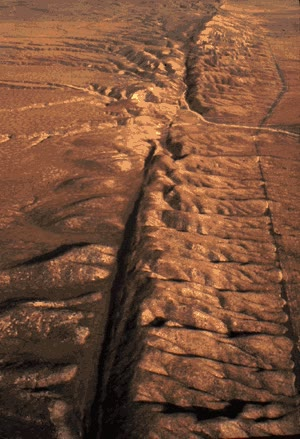
\includegraphics[width=0.28\linewidth]{images/book1/g7-usgs-san-andreas.jpg}

{\small Sesar San Andreas yang melintasi \omterm{def:g1:landscapes-around-us:landform}{Dataran} Carrizo, California,
dilihat dari pesawat terbang: \omterm{def:g1:landscapes-around-us:landform}{lembah} panjang yang lurus itu adalah batas
antara \omterm{def:g7:plate-tectonics:plate}{lempeng} Pasifik (kiri) dan \omterm{def:g7:plate-tectonics:plate}{lempeng} Amerika Utara (kanan). Foto:
Robert E. Wallace, U.S. Geological Survey (domain publik).}
\end{omfigure}

\begin{method}[Mengenali batas lempeng pada peta]\label{met:g7:plate-tectonics:recognise}
Untuk menentukan jenis batas yang memisahkan dua \omterm{def:g7:plate-tectonics:plate}{lempeng}:
\begin{enumerate}
  \item carilah, pada \omterm{def:g2:drawing-to-map:map}{peta} gerak \omterm{def:g7:plate-tectonics:plate}{lempeng}, panah-panah di kedua sisi batas
        itu;
  \item jika panah-panah itu mengarah menjauhi batas, batas itu divergen;
        jika mengarah ke batas, konvergen; jika sejajar dengan batas dan
        mengarah ke arah yang berlawanan, transform;
  \item periksalah dengan \omterm{def:g1:landscapes-around-us:landscape}{bentang alamnya}: punggung di tengah \omterm{def:g2:water-on-earth:ocean}{samudra} atau
        rekahan yang membelah \omterm{def:g3:continents-and-oceans:continent}{benua} menyertai \omterm{def:g7:plate-tectonics:plate-boundary}{batas divergen}; palung dalam
        dengan deretan \omterm{def:g4:volcanoes-earthquakes-first-look:volcano}{gunung api}, atau \omterm{def:g4:world-physical-map:range}{pegunungan} tinggi, menyertai \omterm{def:g7:plate-tectonics:plate-boundary}{batas
        konvergen}; sesar panjang yang lurus tanpa keduanya menyertai \omterm{def:g7:plate-tectonics:plate-boundary}{batas
        transform}.
\end{enumerate}
\end{method}

\section{Seberapa cepat lempeng bergerak?}

\begin{proposition}[Beberapa sentimeter setahun]\label{prop:g7:plate-tectonics:speed}
% ledger: data:pb2002 (speeds computed in figdata/grade-7/plate_speeds.py), usgs:mar-rate
Dua \omterm{def:g7:plate-tectonics:plate}{lempeng} yang bertetangga bergerak relatif satu terhadap yang lain
dengan kecepatan beberapa sentimeter per tahun: dari kira-kira
2 sentimeter per tahun di Atlantik Utara sampai lebih dari 14 sentimeter
per tahun di Punggung Pasifik Timur, punggung \omterm{def:g2:water-on-earth:ocean}{samudra} yang paling cepat
memekar di Bumi.
\end{proposition}

\begin{omfigure}
\begin{tikzpicture}
\begin{axis}[xbar, width=0.74\linewidth, height=5.4cm, xmin=0, xmax=16.5,
  ytick={1,...,6}, yticklabels={punggung Atlantik Utara, punggung Atlantik Selatan,
  Sesar San Andreas, Himalaya, Palung Peru--Chili, Punggung Pasifik Timur},
  y tick label style={font=\small}, tick label style={font=\small},
  xlabel={kecepatan satu lempeng relatif terhadap yang lain (cm per tahun)},
  label style={font=\small}, bar width=7pt, axis x line=bottom,
  axis y line=left, axis line style={-}, enlarge y limits=0.12,
  nodes near coords, nodes near coords style={font=\scriptsize},
  every node near coord/.append style={/pgf/number format/fixed,
  /pgf/number format/precision=1, /pgf/number format/fixed zerofill}]
\addplot[fill=omDef!55, draw=omDef!80!black] table[x=speed_cm_a, y=rank] {figdata/out/grade-7-plate_speeds.dat};
\end{axis}
\end{tikzpicture}

{\small Kecepatan gerak \omterm{def:g7:plate-tectonics:plate}{lempeng} di enam batas: rata-rata di sepanjang setiap
batas, dihitung dari model \omterm{def:g7:plate-tectonics:plate}{lempeng} P.~Bird (2003).}
\end{omfigure}

\begin{method}[Dari sentimeter per tahun ke kilometer per juta tahun]\label{met:g7:plate-tectonics:convert}
Satu kilometer sama dengan \num{100000} sentimeter. Kecepatan \qty{1}{cm}
per tahun, yang berlangsung terus selama sejuta tahun, karena itu menempuh
\num{1000000} sentimeter, yaitu \qty{10}{km}. Jadi:
\[
  1\ \text{cm per tahun} = 10\ \text{km per juta tahun}.
\]
Kalikan kecepatan dalam sentimeter per tahun dengan 10 untuk mendapatkan
kilometer per juta tahun; lalu kalikan dengan sejumlah juta tahun untuk
mendapatkan jarak dalam kilometer, atau bagilah jarak dengan kecepatan itu
untuk mendapatkan waktu.
\end{method}

\begin{example}[Atlantik makin lebar]\label{ex:g7:plate-tectonics:atlantic}
% ledger: usgs:mar-rate
Rata-rata, kedua sisi Punggung Tengah Atlantik saling menjauh kira-kira
\qty{2.5}{cm} per tahun, yaitu \qty{25}{km} per juta tahun. Dalam 100 juta
tahun, jaraknya menjadi \qty{2500}{km}: jika berlangsung cukup lama,
kecepatan yang terlalu lambat untuk disadari seumur hidup ini membuka
sebuah \omterm{def:g2:water-on-earth:ocean}{samudra}.
\end{example}

\begin{remark}[Mengukur gerak itu pada masa kini]\label{rem:g7:plate-tectonics:gps}
% ledger: usgs:gps
Gerak yang selambat itu kini diukur secara langsung. Stasiun-stasiun tetap
yang dipasang pada \omterm{def:g3:stones-pebbles-sand:rock}{batuan dasar} menerima sinyal satelit penentu posisi dan
menghitung posisinya sendiri, hari demi hari, sampai ketelitian beberapa
milimeter. Dalam beberapa tahun, stasiun-stasiun pada \omterm{def:g7:plate-tectonics:plate}{lempeng} yang berbeda
terlihat saling menjauh atau saling mendekat, dengan kecepatan yang sama
dengan yang ditemukan dari \omterm{def:g3:stones-pebbles-sand:rock}{batuan} selama jutaan tahun. Penentuan posisi
dengan satelit itu sendiri dibahas dalam \cref{ch:g9:maps-of-the-earth}.
\end{remark}

\begin{omfigure}
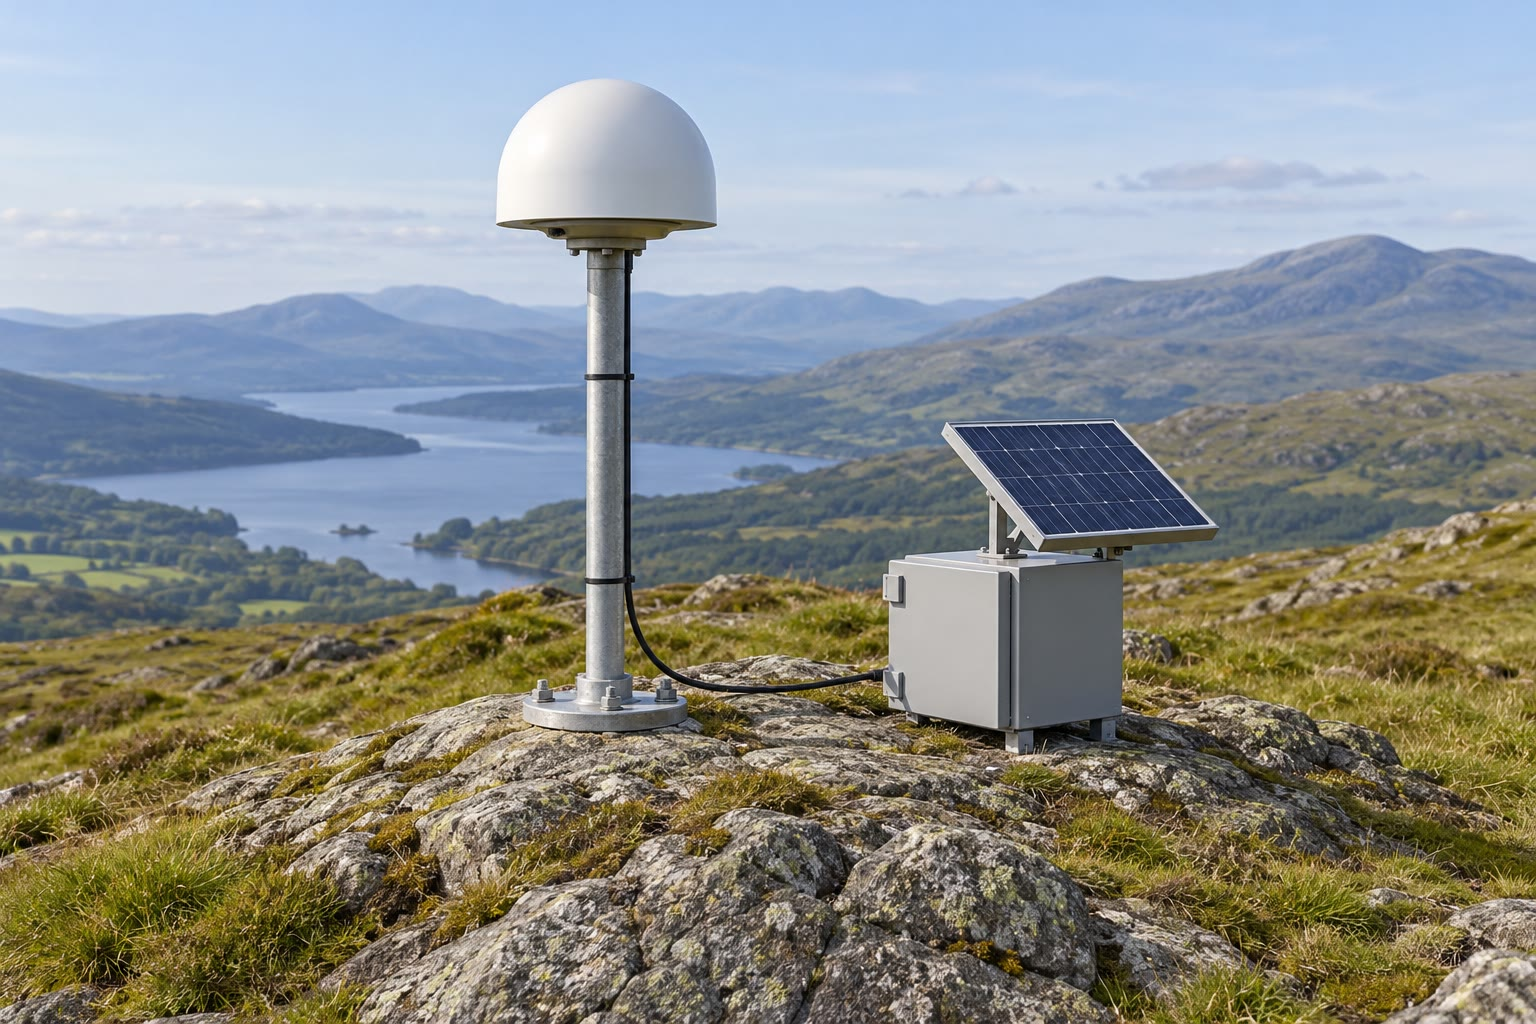
\includegraphics[width=0.55\linewidth]{images/book1/ai/g7-gps-station.jpg}

{\small Sebuah stasiun penentu posisi yang tetap: antenanya dibaut ke
\omterm{def:g3:stones-pebbles-sand:rock}{batuan}, sehingga stasiun itu bergerak bersama \omterm{def:g7:plate-tectonics:plate}{lempengnya}.}
\end{omfigure}

\section{Latihan}

\begin{exercise}[$\star$]\label{exo:g7:plate-tectonics:1}
Apa yang dimaksud dengan \omterm{def:g7:plate-tectonics:continental-drift}{pergeseran benua}? Sebutkan empat jenis petunjuk
yang dipakai Wegener untuk membelanya.
\end{exercise}

\begin{exercise}[$\star$]\label{exo:g7:plate-tectonics:2}
Sebutkan tiga jenis \omterm{def:g7:plate-tectonics:plate-boundary}{batas lempeng} dan jelaskan, untuk setiap jenis,
bagaimana kedua \omterm{def:g7:plate-tectonics:plate}{lempeng} bergerak terhadap satu sama lain.
\end{exercise}

\begin{exercise}[$\star$]\label{exo:g7:plate-tectonics:3}
Perhatikan \omterm{def:g2:drawing-to-map:map}{peta} \omterm{def:g4:volcanoes-earthquakes-first-look:earthquake}{gempa bumi} dan \omterm{def:g4:volcanoes-earthquakes-first-look:volcano}{gunung api}. Sebutkan dua wilayah di dunia
yang banyak mengalami \omterm{def:g4:volcanoes-earthquakes-first-look:earthquake}{gempa bumi} besar, dan satu \omterm{def:g3:continents-and-oceans:continent}{benua} yang hampir tidak
mengalaminya di bagian tengahnya.
\end{exercise}

\begin{exercise}[$\star$]\label{exo:g7:plate-tectonics:4}
Fosil \emph{Mesosaurus}, reptil kecil yang hidup di \omterm{def:g2:water-on-earth:salt-fresh}{air tawar}, ditemukan
di Brasil dan di Afrika bagian selatan. Mengapa hal ini merupakan petunjuk
bahwa kedua \omterm{def:g3:continents-and-oceans:continent}{benua} itu dulu menyatu?
\end{exercise}

\begin{exercise}[$\star\star$]\label{exo:g7:plate-tectonics:5}
Batu bara ditemukan di Antarktika. Apa yang ditunjukkan hal ini tentang
\omterm{def:g5:weather-and-climate:climate}{iklim} tempat batu bara itu terbentuk, dan apa yang dapat kita simpulkan
tentang letak Antarktika pada waktu itu?
\end{exercise}

\begin{exercise}[$\star\star$]\label{exo:g7:plate-tectonics:6}
Sebutkan jenis batas yang terdapat di setiap tempat berikut: Punggung
Tengah Atlantik; \omterm{def:g4:world-physical-map:range}{Pegunungan} Andes; Sesar San Andreas; Himalaya; Rekahan
Afrika Timur.
\end{exercise}

\begin{exercise}[$\star\star$]\label{exo:g7:plate-tectonics:7}
Ubahlah kecepatan \qty{2.5}{cm} per tahun menjadi kilometer per juta tahun.
Seberapa jauh dua titik di kedua sisi batas akan saling menjauh dalam 60
juta tahun dengan kecepatan ini?
\end{exercise}

\begin{exercise}[$\star\star$]\label{exo:g7:plate-tectonics:8}
Antara tahun 1975 dan 1984 --- sembilan tahun --- retakan-retakan di dekat
\omterm{def:g4:volcanoes-earthquakes-first-look:volcano}{gunung api} Krafla di Islandia melebar kira-kira \qty{7}{m} seluruhnya.
Berapa rata-rata pelebarannya per tahun, dalam sentimeter? Bandingkan
dengan kecepatan rata-rata Punggung Tengah Atlantik, kira-kira
\qty{2.5}{cm} per tahun, dan kemukakan mengapa kedua bilangan itu sangat
berbeda.
\end{exercise}

\begin{exercise}[$\star\star$]\label{exo:g7:plate-tectonics:9}
Teori Wegener ditolak selama puluhan tahun. Pertanyaan apa yang tidak dapat
dijawabnya? Apa yang diubah oleh teori \omterm{def:g7:plate-tectonics:plate-tectonics}{tektonika lempeng} dalam gambarannya
tentang \omterm{def:g3:continents-and-oceans:continent}{benua-benua} yang bergerak?
\end{exercise}

\begin{exercise}[$\star\star$]\label{exo:g7:plate-tectonics:10}
Perhatikan penampang melintang dua \omterm{def:g7:plate-tectonics:plate-boundary}{batas lempeng}. Di mana dasar \omterm{def:g2:water-on-earth:ocean}{laut} paling
tinggi, dan di mana paling dalam? Di mana \omterm{def:g7:plate-tectonics:plate}{lempeng} baru sedang dibuat, dan di
mana sebuah \omterm{def:g7:plate-tectonics:plate}{lempeng} kembali ke dalam \omterm{def:g6:inside-the-earth:layers}{mantel}?
\end{exercise}

\begin{exercise}[$\star\star\star$]\label{exo:g7:plate-tectonics:11}
Di Punggung Pasifik Timur, \omterm{def:g7:plate-tectonics:plate}{lempeng-lempeng} saling menjauh kira-kira
\qty{14.2}{cm} per tahun, dan di punggung Atlantik Utara kira-kira
\qty{2.2}{cm} per tahun. Berapa kali lebih cepat Punggung Pasifik Timur
(bulatkan ke bilangan bulat terdekat)? Berapa lama waktu yang diperlukan
setiap punggung untuk membuka dasar \omterm{def:g2:water-on-earth:ocean}{samudra} baru selebar \qty{1000}{km}?
\end{exercise}

\begin{exercise}[$\star\star\star$]\label{exo:g7:plate-tectonics:12}
% ledger: data:usgs-comcat, data:pb2002 (counts in figdata/grade-7/quakes_on_boundaries.py, part bands)
Dari 7\,031 \omterm{def:g4:volcanoes-earthquakes-first-look:earthquake}{gempa bumi} bermagnitudo 6 atau lebih yang tercatat dari tahun
1976 sampai 2025, 4\,578 terjadi kurang dari \qty{100}{km} dari garis \omterm{def:g7:plate-tectonics:plate-boundary}{batas
lempeng} yang digambar pada \omterm{def:g2:drawing-to-map:map}{peta}, 6\,472 kurang dari \qty{300}{km}, dan
6\,786 kurang dari \qty{500}{km}.
(a) Berapa banyak yang terjadi antara \qty{100}{km} dan \qty{300}{km} dari
garis itu? (b) Hitunglah, dibulatkan ke bilangan bulat terdekat, persentase
\omterm{def:g4:volcanoes-earthquakes-first-look:earthquake}{gempa bumi} yang terjadi kurang dari \qty{100}{km} dari garis itu terhadap
seluruh \omterm{def:g4:volcanoes-earthquakes-first-look:earthquake}{gempa bumi} ini. (c) Banyak \omterm{def:g4:volcanoes-earthquakes-first-look:earthquake}{gempa bumi} yang berjarak antara
\qty{100}{km} dan \qty{300}{km} dari garis itu terletak pada sisi yang sama
dari sebuah palung \omterm{def:g2:water-on-earth:ocean}{samudra} yang dalam. Dengan memakai apa yang terjadi pada
\omterm{def:g7:plate-tectonics:plate-boundary}{batas konvergen}, jelaskan mengapa \omterm{def:g4:volcanoes-earthquakes-first-look:earthquake}{gempa bumi} yang disebabkan oleh sebuah
\omterm{def:g7:plate-tectonics:plate-boundary}{batas lempeng} dapat terjadi sejauh itu dari garis yang digambar pada \omterm{def:g2:drawing-to-map:map}{peta}.
\end{exercise}

\section{Soal: Terbukanya Atlantik Selatan}

\begin{problem}[{Soal akhir pekan --- mengukur sebuah samudra pada peta dan
mencari berapa lama samudra itu terbuka}]
\label{pb:g7:plate-tectonics:1}
% ledger: data:ne-land, earth:Rmean, data:pb2002, usgs:pangaea-breakup, usgs:atlantic-growth
% (all numbers computed in figdata/grade-7/south_atlantic.py: coasts at 23 S
% at 43.21 W and 14.39 E, 102.4 km per degree, AF-SA full rate 3.43 cm/yr)
Pada \omterm{def:g2:drawing-to-map:map}{peta} Atlantik Selatan, seorang siswa mengikuti \omterm{def:g6:latitude-longitude:latitude}{paralel}
\ang{23}\,LS. \omterm{def:g6:latitude-longitude:latitude}{Paralel} itu meninggalkan pantai Amerika Selatan di dekat Rio
de Janeiro, pada \omterm{def:g6:latitude-longitude:longitude}{bujur} \ang{43.2}\,BB, menyeberangi \omterm{def:g2:water-on-earth:ocean}{samudra} dan Punggung
Tengah Atlantik, lalu mencapai pantai Afrika di dekat Walvis Bay, pada
\omterm{def:g6:latitude-longitude:longitude}{bujur} \ang{14.4}\,BT. Pada \omterm{def:g6:latitude-longitude:latitude}{paralel} ini, satu derajat \omterm{def:g6:latitude-longitude:longitude}{bujur} panjangnya
\qty{102}{km}. Di punggung \omterm{def:g2:water-on-earth:ocean}{samudra} itu, pada \omterm{def:g6:latitude-longitude:latitude}{lintang} ini, \omterm{def:g7:plate-tectonics:plate}{lempeng} Amerika
Selatan dan \omterm{def:g7:plate-tectonics:plate}{lempeng} Afrika saling menjauh dengan kecepatan \qty{3.4}{cm}
per tahun.

\begin{center}
\begin{tikzpicture}
\begin{axis}[axis equal image, xmin=-60, xmax=30, ymin=-42, ymax=12,
  width=0.6\linewidth, tick label style={font=\scriptsize},
  xtick={-60,-40,...,20}, ytick={-40,-20,0},
  xticklabel={$\pgfmathprintnumber{\tick}^\circ$},
  yticklabel={$\pgfmathprintnumber{\tick}^\circ$},
  axis background/.style={fill=omSea}]
\addplot[fill=omLithAlluv, draw=black!45, line width=0.3pt] table {figdata/out/shared-geo-land.dat};
\addplot[omRidge, line width=0.9pt, unbounded coords=jump, restrict x to domain=-45:5] table {figdata/out/shared-geo-school-ridge.dat};
\addplot[omRidge!70!black, line width=0.9pt, unbounded coords=jump, restrict x to domain=-45:5] table {figdata/out/shared-geo-school-transform.dat};
\draw[black, densely dashed, line width=0.7pt] (axis cs:-43.21,-23) -- (axis cs:14.39,-23);
\fill (axis cs:-43.21,-23) circle (1.5pt);
\fill (axis cs:14.39,-23) circle (1.5pt);
\node[font=\scriptsize, below right, inner sep=2pt] at (axis cs:-43.21,-23) {Rio de Janeiro};
\node[font=\scriptsize, below left, inner sep=2pt] at (axis cs:14.39,-23) {Walvis Bay};
\node[font=\scriptsize, anchor=east, inner sep=1pt] at (axis cs:-16.5,-34) {Punggung Tengah Atlantik};
\end{axis}
\end{tikzpicture}
\end{center}

\medskip
\noindent\textbf{Bagian I --- Petunjuk dari kecocokan.}
\begin{enumerate}
  \item Pada \omterm{def:g2:drawing-to-map:map}{peta} fosil dalam bab ini, sebutkan fosil-fosil yang pitanya
        menyeberang dari Amerika Selatan ke Afrika.
  \item Mengapa fosil \emph{Mesosaurus} tidak dapat dijelaskan oleh hewan
        yang berenang dari satu \omterm{def:g3:continents-and-oceans:continent}{benua} ke \omterm{def:g3:continents-and-oceans:continent}{benua} yang lain?
  \item Bagian Amerika Selatan yang mana yang cocok dengan bagian Afrika
        yang mana?
  \item Jenis \omterm{def:g7:plate-tectonics:plate-boundary}{batas lempeng} apa yang membentang di tengah-tengah Atlantik
        Selatan pada masa kini? Bagaimana kedua \omterm{def:g7:plate-tectonics:plate}{lempeng} bergerak di sana?
\end{enumerate}

\medskip
\noindent\textbf{Bagian II --- Mengukur samudra.}
\begin{enumerate}[resume]
  \item Berapa derajat \omterm{def:g6:latitude-longitude:longitude}{bujur} yang memisahkan kedua pantai di sepanjang
        \omterm{def:g6:latitude-longitude:latitude}{paralel} \ang{23}\,LS?
  \item Berapa lebar \omterm{def:g2:water-on-earth:ocean}{samudra} itu, dalam kilometer, di sepanjang \omterm{def:g6:latitude-longitude:latitude}{paralel}
        ini? Bulatkan ke puluhan kilometer terdekat.
  \item Di \omterm{def:g3:continents-and-oceans:equator}{khatulistiwa}, satu derajat \omterm{def:g6:latitude-longitude:longitude}{bujur} panjangnya \qty{111}{km}.
        Mengapa panjangnya hanya \qty{102}{km} pada \ang{23}\,LS?
  \item Punggung \omterm{def:g2:water-on-earth:ocean}{samudra} itu membentang kira-kira di tengah-tengah \omterm{def:g2:water-on-earth:ocean}{samudra}.
        Kira-kira seberapa jauh setiap pantai dari punggung itu?
\end{enumerate}

\medskip
\noindent\textbf{Bagian III --- Umur samudra.}
\begin{enumerate}[resume]
  \item Ubahlah kecepatan saling menjauhnya kedua \omterm{def:g7:plate-tectonics:plate}{lempeng} itu menjadi
        kilometer per juta tahun.
  \item Seandainya \omterm{def:g2:water-on-earth:ocean}{samudra} itu selalu terbuka dengan kecepatan ini, berapa
        juta tahun yang diperlukan untuk mencapai lebarnya yang sekarang?
        Bulatkan ke puluhan juta tahun terdekat.
  \item Para ahli geologi menentukan bahwa \omterm{def:g7:plate-tectonics:supercontinent}{Pangea} terpecah antara kira-kira
        225 dan 200 juta tahun yang lalu, dan menyatakan bahwa Atlantik telah
        melebar selama 100 sampai 200 juta tahun terakhir. Apakah jawabanmu
        sesuai dengan hal ini?
  \item Berikan satu alasan mengapa umur Atlantik Selatan yang sebenarnya
        dapat berbeda dari umur yang kamu temukan.
\end{enumerate}
\end{problem}
